\documentclass[12pt, letterpaper]{article}

\usepackage[utf8]{inputenc}
\usepackage[T1]{fontenc}
\usepackage[spanish, es-tabla]{babel}
\usepackage{mathptmx} % Times New Roman clasica de la escuela
\usepackage{geometry}
\usepackage{setspace}
\usepackage{graphicx}
\usepackage{booktabs}
\usepackage{array}
\usepackage{hanging}
\usepackage{amsmath, amssymb}
\usepackage{url}
\usepackage[hidelinks]{hyperref}

% Margenes estandares UCV (3cm sup/izq, 2.5cm inf/der)
\geometry{
  top=3cm,
  bottom=2.5cm,
  left=3cm,
  right=2.5cm
}

\usepackage{float}
\usepackage{xurl}
\usepackage{tocloft}

% Ajuste de ancho de numeros en el indice para que no choquen los de 2 digitos (10 al 15)
\renewcommand{\cftsecnumwidth}{2.4em}
\renewcommand{\cftsubsecnumwidth}{2.8em}

\onehalfspacing
\setlength{\parindent}{0cm}
\setlength{\parskip}{1.5ex}

% En la EECA-UCV se denomina Cuadro a las tablas
\addto\captionsspanish{
  \renewcommand{\tablename}{Cuadro}
  \renewcommand{\listtablename}{Índice de Cuadros}
}

\begin{document}

% -------------------------------------------------------------
% PORTADA
% -------------------------------------------------------------
\begin{titlepage}
    \centering
    {\bfseries UNIVERSIDAD CENTRAL DE VENEZUELA\\
    FACULTAD DE CIENCIAS ECONÓMICAS Y SOCIALES\\
    ESCUELA DE ESTADÍSTICA Y CIENCIAS ACTUARIALES\\
    DEPARTAMENTO DE INFORMÁTICA\\
    COMPUTACIÓN ESTADÍSTICA\par}
    \vspace{0.3cm}
    {\small SEMESTRE 2026-01S\par}
    
    \vspace{3.2cm}
    {\bfseries\large EL IMPACTO DEL USO DE DISPOSITIVOS ELECTRÓNICOS EN LA CALIDAD DEL SUEÑO DE ESTUDIANTES DE LA EECA-UCV DURANTE EL PERÍODO 2026-01S\par}
    
    \vspace{3.5cm}
    \noindent
    \begin{minipage}[t]{0.55\textwidth}
        \raggedright
        \textbf{Estudiantes:}\\[0.15cm]
        Armando Delfín, C.I: 30.330.804\\
        Giovanni Fermín, C.I: 31.112.857\\
        Anaís Moncada, C.I: 26.152.765
    \end{minipage}%
    \hfill
    \begin{minipage}[t]{0.38\textwidth}
        
        \textbf{Profesora:}\\[0.15cm]
        Oriana Medina
    \end{minipage}
    
    \vfill
    {\normalsize Caracas, Septiembre 2026\par}
\end{titlepage}

% -------------------------------------------------------------
% INDICE DE CONTENIDOS
% -------------------------------------------------------------
\pagenumbering{roman}
\begin{singlespace}
\tableofcontents
\end{singlespace}
\newpage

\pagenumbering{arabic}
\setcounter{page}{1}

% -------------------------------------------------------------
% CUERPO DEL ANTEPROYECTO
% -------------------------------------------------------------

\section{Planteamiento del Problema}

Desde la popularización y uso masivo de la tecnología en información y comunicación móvil, se ha visto una mutación sustancial en los hábitos de la cotidianidad de la población en todo el mundo (LeBourgeois et al., 2017). Particularmente en los jóvenes, quienes representan la mayor proporción estudiantil en los sectores de educación superior; quienes han adoptado de forma masiva el uso de los dispositivos móviles en la rutina diaria, tanto diurna como nocturna.

El uso recurrente de estos dispositivos es capaz de impactar la calidad del sueño a través de varios mecanismos (LeBourgeois et al., 2017): la sustitución del tiempo invertido en otras actividades para en cambio invertirlo en el uso de pantallas, el estímulo psicológico derivado del contenido digital y la emisión de luz azul, la cual puede tener un impacto en el ciclo circadiano. Esto es preocupante, pues tener hábitos de sueño saludables es fundamental para tener una buena salud (Hirshkowitz et al., 2015). Sin embargo, en los últimos años se ha observado un declive significativo en la cantidad de horas de sueño promedio en todo el mundo, siendo que para el 2015 la proporción de adultos durmiendo habitualmente menos del rango óptimo de 7 a 9 horas es de uno por cada tres (Liu et al., 2016).

En el contexto local y objetivo de estudio, la Escuela de Estadística y Ciencias Actuariales de la Universidad Central de Venezuela (EECA-UCV), las asignaturas representan una alta carga cognitiva y un alto grado de dedicación al cómputo y uso de dispositivos móviles, la búsqueda de información y métodos de estudio digitales fomentan el uso de estos dispositivos. Durante el período académico 2026-01S (y en anteriores períodos), la comunidad estudiantil enfrenta estas presiones de carácter logístico, lo que incrementa el uso de los dispositivos electrónicos en horarios poco convencionales.

La falta de un diagnóstico estadístico formal sobre la persistencia de este comportamiento y su vinculación con los trastornos en patrones de descanso, limita el desarrollo de técnicas y estrategias de salud. Por lo tanto, se plantea la siguiente interrogante: ¿Existe un impacto estadísticamente significativo del tiempo invertido en el uso de dispositivos electrónicos y los hábitos de uso en períodos nocturnos sobre la calidad y duración efectiva del sueño en los estudiantes inscritos en la EECA-UCV durante el semestre 2026-01S?


\section{Objetivos de la Investigación}

\subsection{Objetivo General}
Evaluar de manera cuantitativa el impacto del uso de los dispositivos electrónicos durante períodos nocturnos sobre la calidad y la duración del sueño de los estudiantes de la Escuela de Estadística y Ciencias Actuariales de la Universidad Central de Venezuela (EECA-UCV) durante el período lectivo 2026-01S.

\subsection{Objetivos Específicos}
\begin{enumerate}
    \item Caracterizar los hábitos de uso de dispositivos electrónicos en los estudiantes de la EECA durante las horas previas al descanso, considerando variables de exposición temporal, tipos de dispositivos y actividades de interacción digital.
    \item Estimar de forma indirecta la duración del sueño de los estudiantes, diferenciando el comportamiento de los sujetos en la semana laboral y en los días de descanso a partir del registro de la hora de acostarse y la hora de levantarse.
    \item Evaluar el nivel percibido de la calidad del sueño e interrupciones del mismo sobre la población de estudio mediante escalas ordinales adaptadas.
    \item Determinar la existencia de asociaciones estadísticas significativas entre las horas calculadas de descanso y la frecuencia o intensidad del uso de los dispositivos mediante tablas de contingencia y análisis descriptivo.
\end{enumerate}


\section{Finalidad}

El propósito central de este trabajo es aportar evidencia empírica directa sobre la realidad estudiantil de la Escuela de Estadística y Ciencias Actuariales, midiendo el impacto que tiene la exposición nocturna a pantallas sobre el descanso diario (LeBourgeois et al., 2017). Más allá de la tarea académica, se busca que los resultados de esta investigación sean de utilidad para la propia escuela, tanto a nivel estudiantil como del profesorado, por ejemplo: diseñar campañas concretas de higiene del sueño, proveer pautas realistas para la administración del tiempo de pantalla en semanas de alta carga evaluativa y abrir espacios de diálogo sobre el balance tecnológico en la vida universitaria.


\section{Justificación}

El descanso nocturno no constituye un simple intervalo de inactividad, sino un proceso neurobiológico activo indispensable para la consolidación sináptica, la memoria de trabajo y la recuperación metabólica (Hirshkowitz et al., 2015). En el ámbito de la EECA-UCV, donde el rendimiento del estudiante se basa principalmente en mantener una concentración sostenida por largos períodos de tiempo frente a asignaturas de alta exigencia analítica (como en Matemáticas, Estadísticas, Probabilidades etc.), la privación de sueño deteriora directamente la agilidad mental de los estudiantes y eleva el margen de error en el razonamiento cuantitativo, principamente durantes semanas de alta carga académica.

En el plano metodológico, esta investigación brinda un valor formativo directo al permitir recolectar datos empíricos de primera mano en el campus estudiantil mediante un cuestionario estructurado, aplicando pruebas de asociación, tabulación cruzada y control de sesgos de medición en lugar de trabajar con conjuntos de datos secundarios. En el plano comunitario, atiende un hábito generalizado entre los estudiantes universitarios: retrasar el horario de dormir para compensar jornadas académicas o extender la interacción en redes sociales (LeBourgeois et al., 2017; Maurya et al., 2022), asumiendo un déficit biológico acumulativo cuyas consecuencias rara vez se cuantifican formalmente, o siquiera se tienen en cuenta.


\section{Cobertura}

\subsection{Cobertura Horizontal}
La investigación está dirigida a los estudiantes de la EECA inscritos durante el período lectivo 2026-01S. El alcance real del estudio dependerá de una muestra conformada por aquellos estudiantes que decidan participar de forma voluntaria mediante su consentimiento.

\subsection{Cobertura Vertical}
Se analizarán los hábitos de uso nocturno de pantallas (con énfasis en teléfonos inteligentes y computadoras portátiles) en las horas previas a dormir, así como la duración estimada del sueño que será calculada a partir de la diferencia entre los horarios de acostarse y levantarse, y la frecuencia de interrupciones del descanso reportadas por los propios estudiantes.


\section{Período de Referencia}

El período para la recolección de los datos y la referencia temporal de las preguntas del cuestionario corresponden al semestre académico activo 2026-01S.


\section{Antecedentes}

El estudio del impacto de las tecnologías en el descanso se fundamenta en investigaciones internacionales previas:

\begin{itemize}
    \item \textbf{He et al. (2025):} En una revisión sistemática y metaanálisis publicada en \textit{Frontiers in Psychiatry} (con 21 estudios de cohorte y más de 548.000 participantes), concluyeron que cada hora adicional de pantalla al día reduce entre 3 y 5 minutos la duración del sueño e incrementa significativamente el riesgo de insomnio.
    \item \textbf{Hysing et al. (2015):} En un estudio poblacional con adolescentes noruegos (\textit{BMJ Open}), determinaron que el uso de computadoras y teléfonos inteligentes antes de acostarse se asocia directamente con un mayor retraso para quedarse dormido y una menor cantidad total de horas de sueño.
    \item \textbf{LeBourgeois et al. (2017):} Revisaron en \textit{Pediatrics} la evidencia disponible y definieron los tres mecanismos mediante los cuales las pantallas perjudican el descanso: la sustitución del tiempo de dormir, la estimulación psicológica provocada por los contenidos y la alteración del ciclo circadiano por la emisión de luz azul.
    \item \textbf{Maurya et al. (2022):} En una investigación con jóvenes publicada en \textit{BMC Public Health}, encontraron que superar las tres horas diarias de uso de pantallas eleva de manera considerable la probabilidad de sufrir dificultades para dormir.
    \item \textbf{Zhong et al. (2025):} Mediante un estudio observacional en adultos publicado en \textit{JAMA Network Open}, demostraron que la interacción con dispositivos electrónicos en la hora previa a dormir se vincula con un descanso más corto y una peor calidad percibida del sueño.
\end{itemize}


\section{Marco Teórico Referencial}

\subsection{Bases Teóricas}

La regulación del sueño humano se explica principalmente a través del modelo de dos procesos (Borbély, 1982; LeBourgeois et al., 2017):

\begin{enumerate}
    \item \textbf{Proceso C (Circadiano):} Es un ciclo biológico interno que dura aproximadamente 24 horas y es regulado por el núcleo supraquiasmático, el cual sincroniza los ritmos de vigilia y descanso guiándose por la luz ambiental captada por la retina.
    \item \textbf{Proceso S (Homeostático):} Es la presión acumulativa de sueño que se incrementa de forma progresiva a medida que transcurren las horas de vigilia continua desde el último despertar.
\end{enumerate}

\textbf{Interacción con la tecnología:} El uso nocturno de pantallas afecta ambos procesos a través de las tres vías descritas en la literatura (LeBourgeois et al., 2017): el primero, es el desplazamiento del horario de dormir al preferir continuar usando el dispositivo; el segundo, es la estimulación psicológica generada por la interacción en redes sociales o contenidos digitales; y el tercero, la exposición directa a la luz azul (450--480 nm), la cual inhibe la liberación de melatonina y retrasa la fase circadiana normal.

\textbf{Higiene del sueño y latencia:} La higiene del sueño engloba los hábitos y condiciones del entorno que facilitan un descanso reparador y continuo (Hirshkowitz et al., 2015). El uso de dispositivos móviles en la cama incrementa la latencia del sueño (el tiempo que transcurre entre acostarse e iniciar el descanso), fragmentando la rutina nocturna y disminuyendo la eficiencia total del sueño (Hysing et al., 2015).


\section{Bases Legales}

La investigación se enmarca en la normativa jurídica venezolana vigente, orientada a la protección de la salud integral, el rendimiento educativo y el tratamiento ético de los datos estadísticos:

\begin{itemize}
    \item \textbf{Constitución de la República Bolivariana de Venezuela (1999):}
    \begin{itemize}
        \item \textit{Artículo 83:} Define la salud como un derecho social fundamental y obligación del Estado, respaldando la necesidad de investigar y prevenir factores que comprometan el bienestar de los jóvenes estudiantes.
        \item \textit{Artículo 84:} Promueve la prevención de enfermedades y el desarrollo de investigaciones orientadas a la salud pública y colectiva.
    \end{itemize}
    
    \item \textbf{Ley Orgánica de Educación (2009):}
    \begin{itemize}
        \item \textit{Artículo 3:} Establece el pleno desarrollo de la personalidad y el bienestar integral como principios de la educación. El descanso adecuado es indispensable para que los estudiantes de la EECA-UCV mantengan un rendimiento académico óptimo ante las altas exigencias de su carrera.
    \end{itemize}
    
    \item \textbf{Ley de la Función Pública de Estadística (2001):}
    \begin{itemize}
        \item \textit{Principio de Confidencialidad y Secreto Estadístico:} Garantiza que toda la información individual aportada por los estudiantes en los cuestionarios sea tratada con fines estrictamente académicos, bajo reserva y resguardando el anonimato de los participantes.
    \end{itemize}
\end{itemize}


\section{Variables en Estudio}

\begin{enumerate}
    \item \textbf{Tiempo de uso nocturno de dispositivos electrónicos (Variable Independiente principal):} Tiempo promedio (en minutos u horas) que el estudiante dedica a pantallas digitales en las horas previas a dormir. \textit{(Cuantitativa continua, escala de razón).}
    \item \textbf{Tipo de dispositivo principal utilizado antes de dormir (Variable Independiente secundaria):} Equipo tecnológico que el estudiante emplea con mayor frecuencia antes del descanso (teléfono inteligente, computadora portátil, tablet u otro). \textit{(Cualitativa nominal politómica).}
    \item \textbf{Duración estimada del sueño (Variable Dependiente):} Total de horas de descanso por noche, calculada a partir de la diferencia entre la hora de acostarse y la hora de levantarse. \textit{(Cuantitativa continua, escala de razón).}
    \item \textbf{Percepción de la calidad del sueño (Variable Dependiente principal):} Valoración subjetiva del descanso expresada por el estudiante mediante una escala Likert (1 = Muy mala a 5 = Muy buena). \textit{(Cualitativa ordinal).}
    \item \textbf{Frecuencia de interrupciones nocturnas (Variable Interviniente):} Cantidad habitual de veces que el estudiante se despierta de manera involuntaria durante la noche. \textit{(Cuantitativa discreta / Ordinal).}
\end{enumerate}


\section{Elementos de la Investigación}

\subsection{Universo en Estudio}
El universo de la investigación está conformado por los estudiantes regulares de pregrado activos en la Universidad Central de Venezuela (UCV).

\subsection{Población en Estudio}
La población bajo estudio corresponde al total de estudiantes regulares formalmente inscritos en el período académico 2026-01S en la Escuela de Estadística y Ciencias Actuariales (EECA-UCV).


\section{Plan de Tabulaciones Básicas}

A continuación se presentan los modelos tabulares y las representaciones gráficas preliminares que estructuran la fase piloto del análisis.

\begin{table}[H]
\centering
\caption{Muestra piloto / Ejemplo de distribución de estudiantes según tipo de dispositivo principal y tiempo promedio de uso nocturno.}
\label{cuadro:piloto}
\vspace{0.25cm}
\small
\begin{tabular}{ccccc}
\toprule
\textbf{Estudiante / ID} & \textbf{Dispositivo Principal} & \textbf{Tiempo de uso (min)} & \textbf{Horas de sueño} & \textbf{Calidad (Likert)} \\
\midrule
001 & Teléfono inteligente & 120 & 5.5 & Mala (2) \\
002 & Computadora portátil & 90  & 6.0 & Regular (3) \\
003 & Teléfono inteligente & 150 & 4.5 & Muy mala (1) \\
004 & Tablet               & 45  & 7.0 & Buena (4) \\
005 & Teléfono inteligente & 180 & 5.0 & Mala (2) \\
006 & Televisor / Otros    & 60  & 6.5 & Regular (3) \\
007 & Computadora portátil & 120 & 5.0 & Mala (2) \\
008 & Teléfono inteligente & 210 & 4.0 & Muy mala (1) \\
009 & Tablet               & 30  & 7.5 & Muy buena (5) \\
010 & Teléfono inteligente & 90  & 6.0 & Regular (3) \\
\bottomrule
\end{tabular}
\end{table}

\vspace{0.2cm}

\begin{figure}[H]
\centering
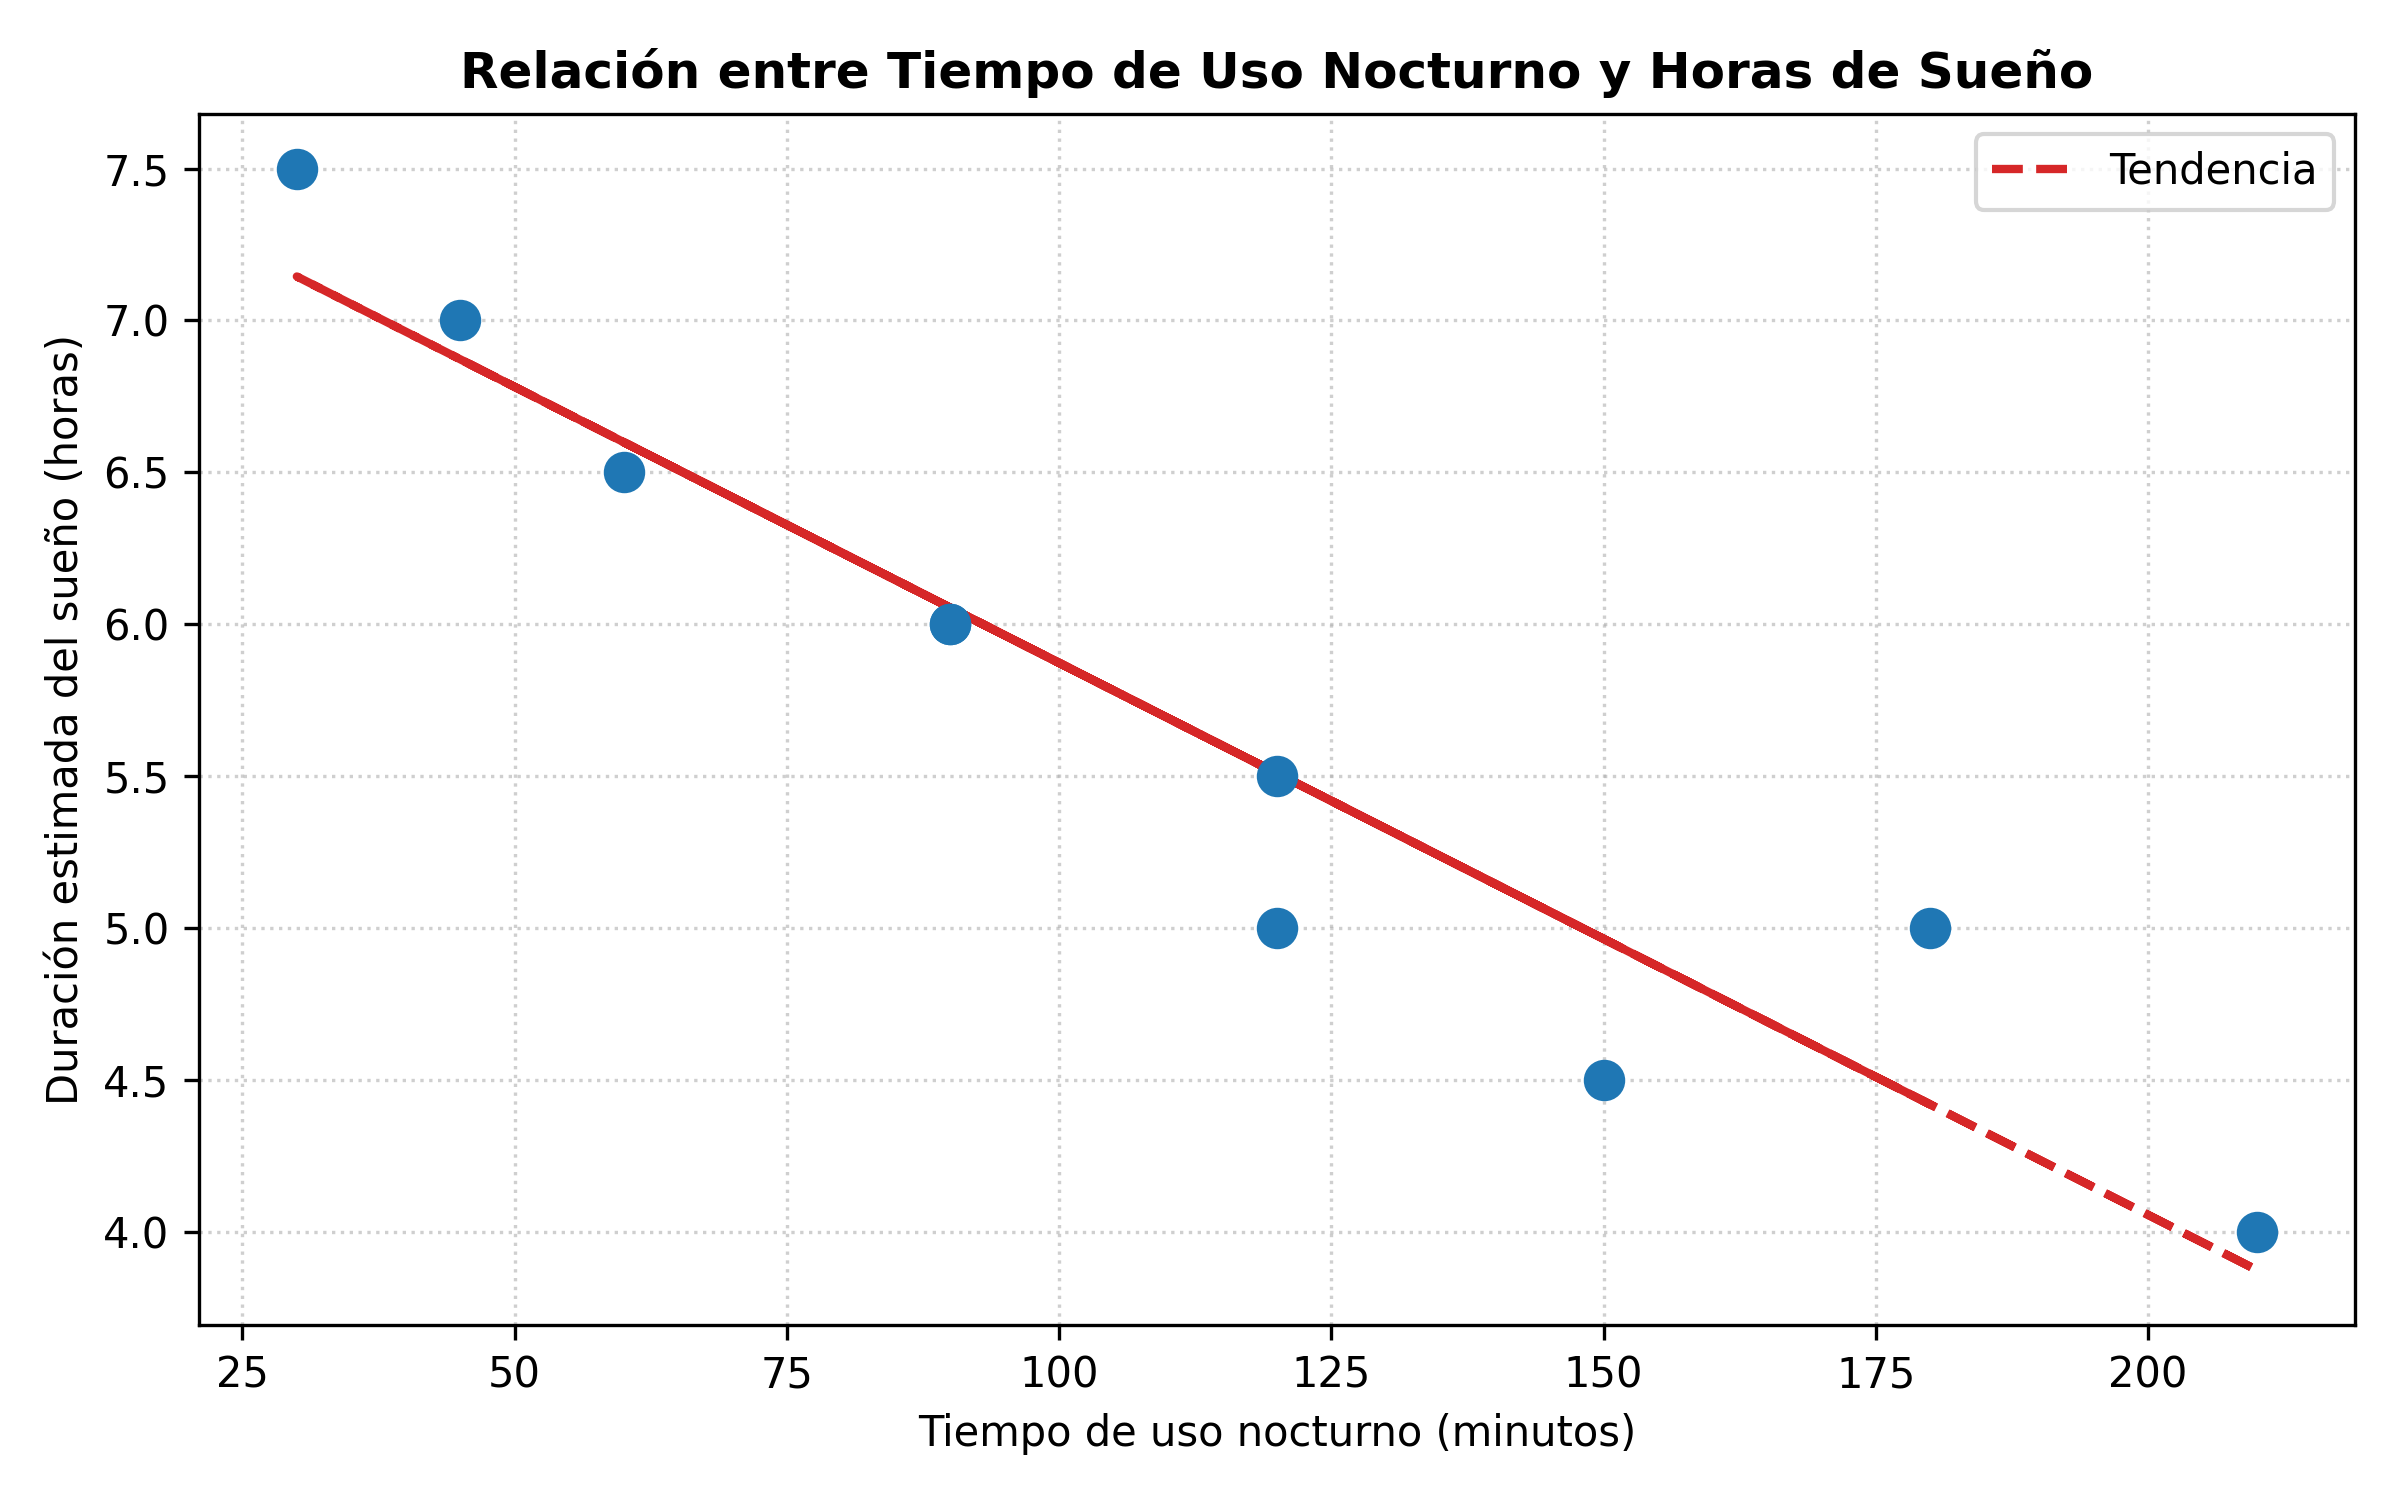
\includegraphics[width=0.82\textwidth]{figura1_dispersion.png}
\caption{Gráfico de dispersión y línea de tendencia entre el tiempo de uso nocturno de pantallas y la duración del sueño, para evaluar si un mayor tiempo frente a la pantalla se asocia con menos horas de descanso.}
\label{fig:dispersion}
\end{figure}

\vspace{0.4cm}

\begin{table}[H]
\centering
\caption{Estadísticas descriptivas de las variables bajo estudio: Tiempo de pantallas y Duración del sueño según prueba piloto/ejemplo.}
\label{cuadro:descriptivas}
\vspace{0.25cm}
\begin{tabular}{lcc}
\toprule
\textbf{Estadísticos} & \textbf{Tiempo de uso nocturno (min)} & \textbf{Duración estimada del sueño (Horas)} \\
\midrule
Media               & 109,50 & 5,70 \\
Mediana             & 105,00 & 5,75 \\
Desviación estándar & 58,33  & 1,11 \\
Mínimo              & 30,00  & 4,00 \\
Máximo              & 210,00 & 7,50 \\
\bottomrule
\end{tabular}
\\[0.25cm]
\parbox{0.88\textwidth}{\footnotesize \textit{Nota:} Parámetros descriptivos calculados sobre la muestra del Cuadro 1 ($n=10$) empleando la cuasivarianza muestral insesgada ($s$).}
\end{table}

\vspace{0.2cm}

\begin{figure}[H]
\centering
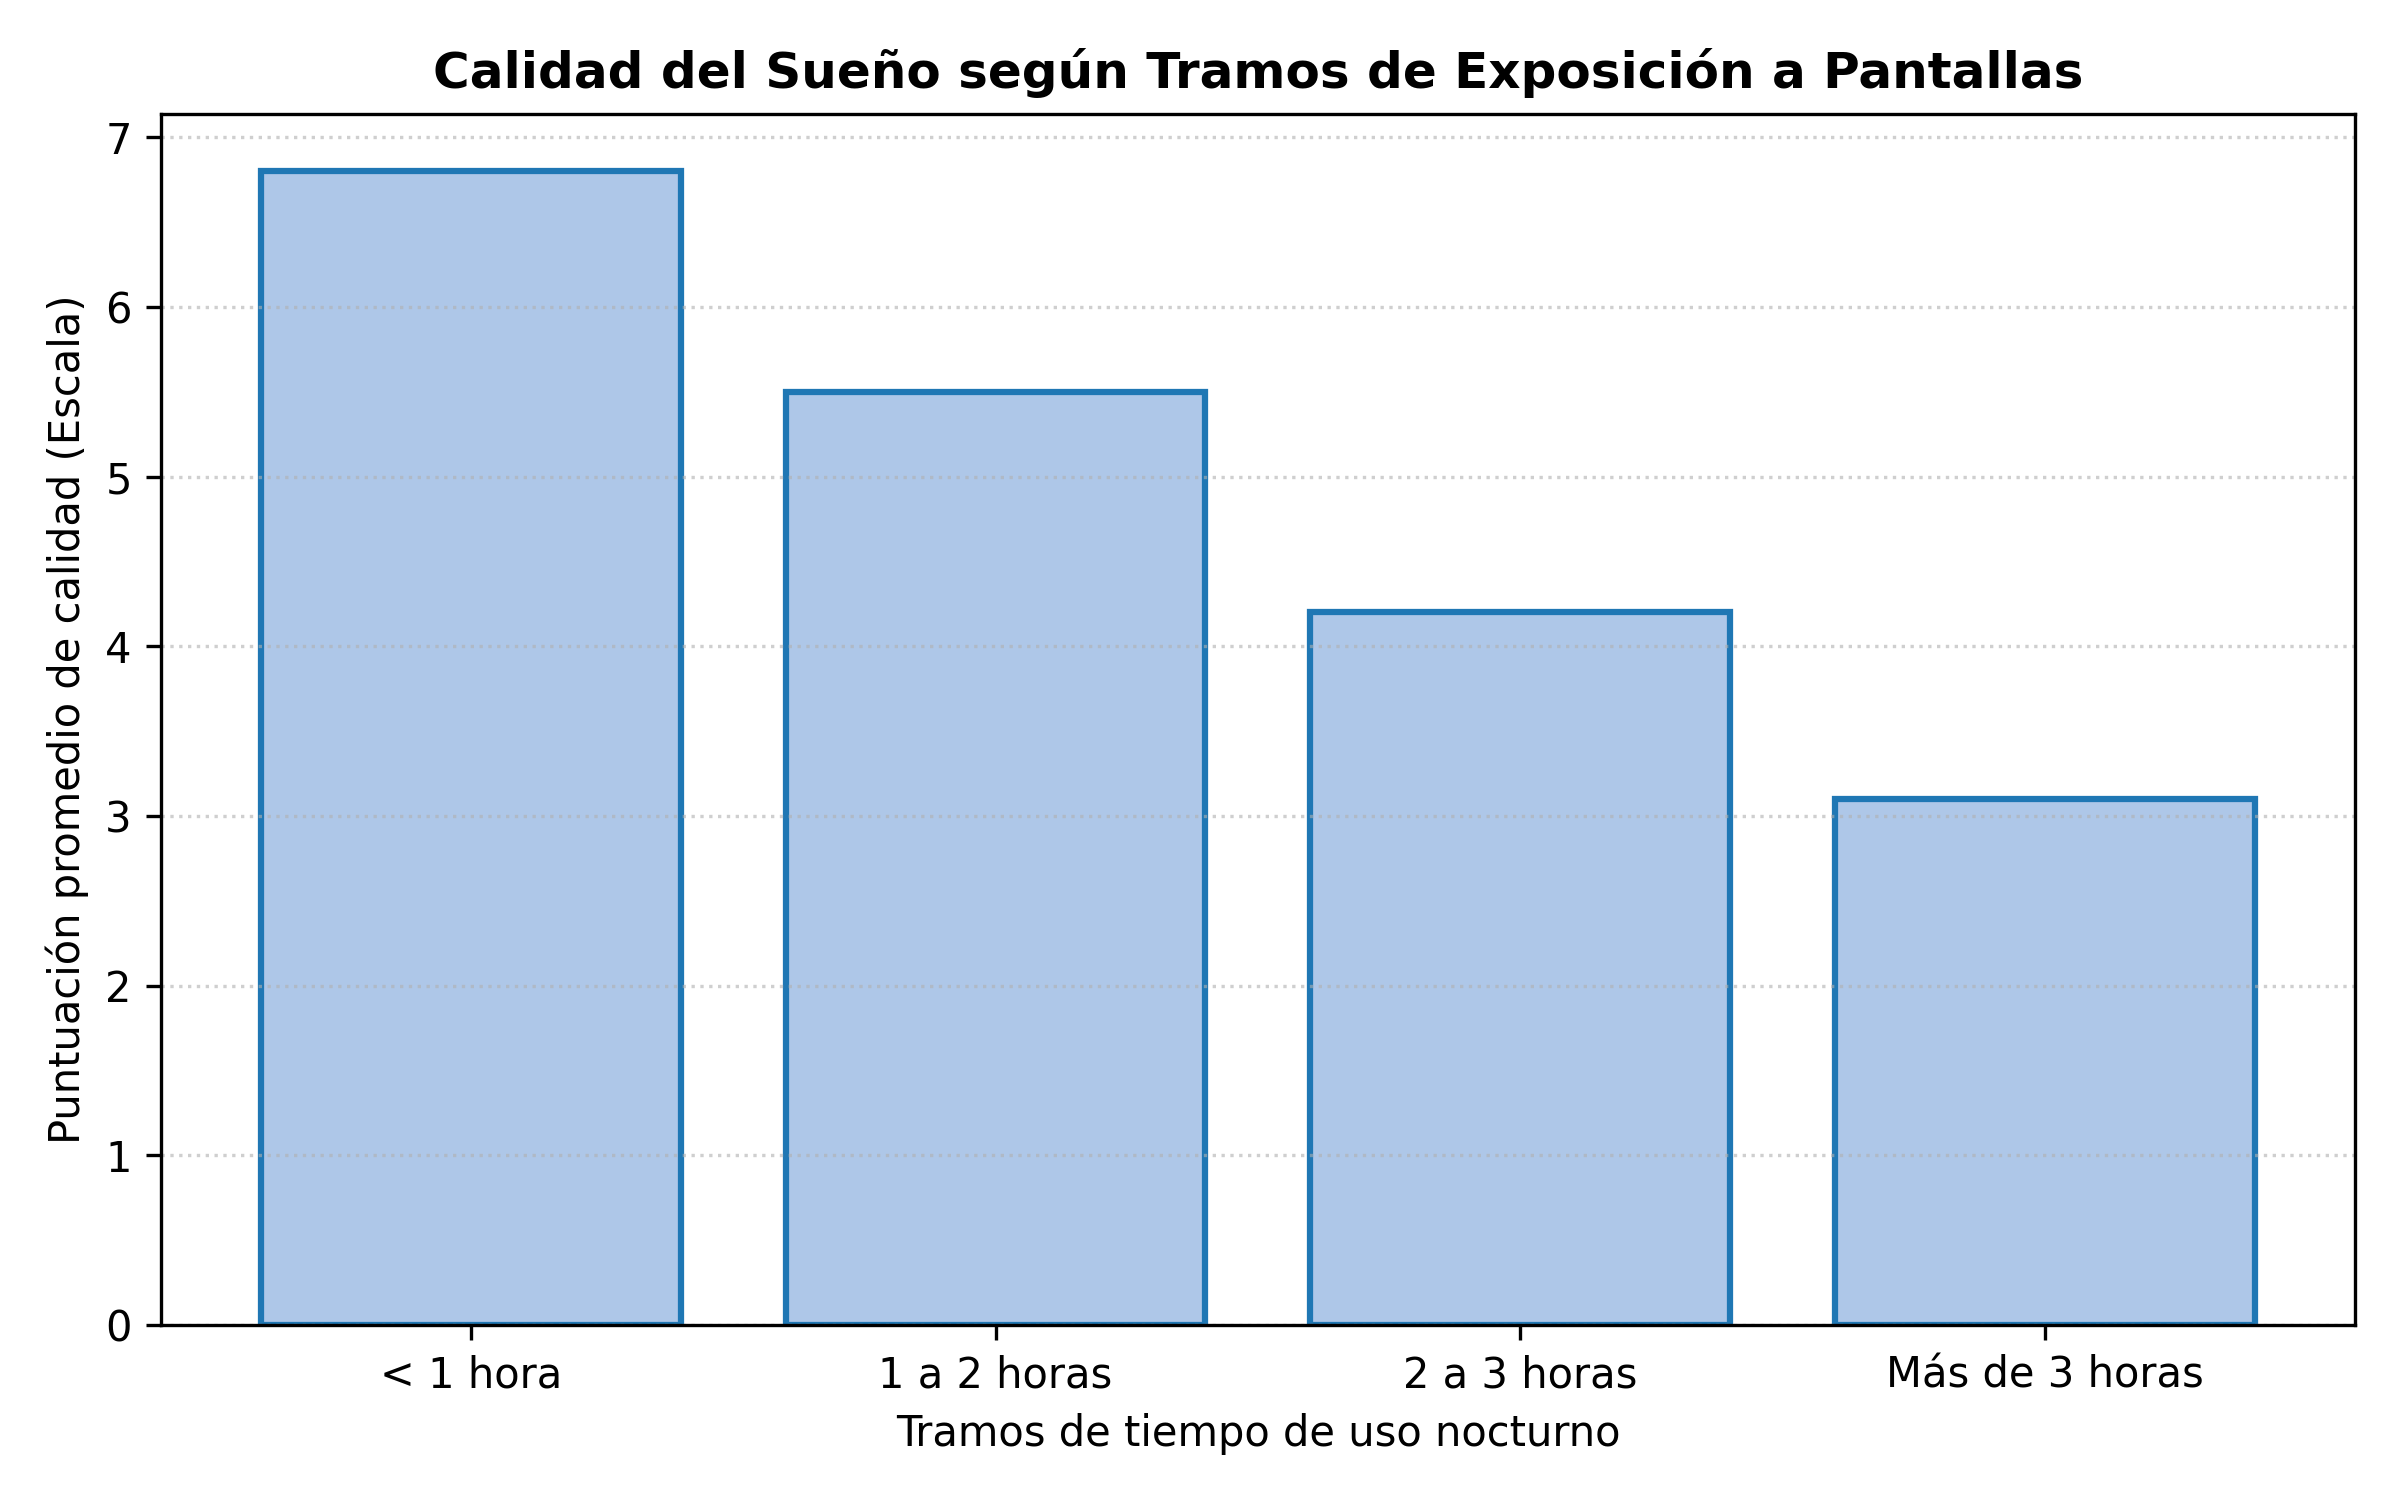
\includegraphics[width=0.82\textwidth]{figura2_descriptivas.png}
\caption{Comparación de las estadísticas descriptivas principales de las variables de estudio (tiempo de exposición a pantallas y duración estimada del sueño).}
\label{fig:descriptivas}
\end{figure}


\section{Cuestionario Preliminar}

\textit{Instrumento aplicado bajo la modalidad de autorreporte digital a la comunidad estudiantil de la EECA-UCV:}

\begin{itemize}
    \item \textbf{Sección I:} Datos Demográficos y Académicos (Género, Semestre).
    \item \textbf{Sección II:} Hábitos de Uso de Dispositivos (Dispositivo principal, Minutos de exposición previa al sueño).
    \item \textbf{Sección III:} Hábitos y Calidad del Sueño (Horarios de acostarse y levantarse en semana y fines de semana, Escala Likert de calidad, Frecuencia de interrupciones).
\end{itemize}


\section{Posibles Dificultades para la Realización del Trabajo}

\begin{enumerate}
    \item \textbf{Inexactitud y sesgo de memoria en el autorreporte:} Al tratarse del uso de la encuesta digital y no de una medición directa del sistema operativo de los teléfonos o los dispositivos electrónicos, los tiempos reportados dependen de la estimación subjetiva de cada estudiante. Esto introduce un margen de error en la reconstrucción retrospectiva del tiempo nocturno, tendiendo a subestimar el uso fragmentado en redes sociales y sobrestimar las horas efectivas dormidas al confundir hora de acostarse con tiempo de sueño real.
    \item \textbf{Caída en la tasa de respuesta por calendarios de evaluación:} La difusión del formulario puede coincidir con momentos álgidos del semestre (períodos de pruebas parciales), lo cual puede mermar la tasa de respuesta voluntaria o concentrar las respuestas en estudiantes con cargas académicas menos exigentes.
    \item \textbf{Variables de confusión no aisladas en el cuestionario:} El descanso universitario se ve condicionado por factores intervinientes de peso como el consumo nocturno de café o estimulantes para estudiar, traslados prolongados hacia la universidad y jornadas laborales extracurriculares o sociales. Aislar con precisión el efecto atribuible exclusivamente a la pantalla requerirá un análisis más cuidadoso.
    \item \textbf{Dispersión por asimetría semanal:} Los estudiantes suelen presentar patrones de descanso bimodal con restricción severa de sueño de lunes a viernes y compensación o desvelo agudo los fines de semana. Al calcular un promedio simple sin diferenciar ambos regímenes distorsionaría la interpretación de la varianza.
\end{enumerate}


\section{Bibliografía}

\begin{hangparas}{.5in}{1}
Borbély, A. A. (1982). A two process model of sleep regulation. \textit{Human Neurobiology}, \textit{1}(3), 195--204.

Constitución de la República Bolivariana de Venezuela. (1999). \textit{Gaceta Oficial de la República Bolivariana de Venezuela Extraordinaria N° 5.453}, 24 de marzo de 2000. \url{http://historico.tsj.gob.ve/legislacion/constitucion1999.htm}

He, X., Pan, B., Ma, N., Li, D., Kong, W., Liu, Q., Liu, X., Wang, X., Deng, X., \& Yang, K. (2025). The association of screen time and the risk of sleep outcomes: A systematic review and meta-analysis. \textit{Frontiers in Psychiatry}, \textit{16}, 1640263. \url{https://www.frontiersin.org/journals/psychiatry/articles/10.3389/fpsyt.2025.1640263/full}

Hirshkowitz, M., Whiton, K., Albert, S. M., Alessi, C., Bruni, O., DonCarlos, L., Hazen, N., Herman, J., Katz, E. S., Kheirandish-Gozal, L., Neubauer, D. N., O'Donnell, A. E., Ohayon, M., Peever, J., Rawding, R., Sachdeva, R. C., Setters, B., Vitiello, M. V., Ware, J. C., \& Adams Hillard, P. J. (2015). National Sleep Foundation's sleep time duration recommendations: Methodology and results summary. \textit{Sleep Health}, \textit{1}(1), 40--43. \url{https://doi.org/10.1016/j.sleh.2014.12.010}

Hysing, M., Pallesen, S., Stormark, K. M., Jakobsen, R., Lundervold, A. J., \& Sivertsen, B. (2015). Sleep and use of electronic devices in adolescence: Results from a large population-based study. \textit{BMJ Open}, \textit{5}(1), e006748. \url{https://bmjopen.bmj.com/content/5/1/e006748}

LeBourgeois, M. K., Hale, L., Chang, A. M., Akacem, L. D., Montgomery-Downs, H. E., \& Buxton, O. M. (2017). Digital media and sleep in childhood and adolescence. \textit{Pediatrics}, \textit{140}(Suppl 2), S92--S96. \url{https://publications.aap.org/pediatrics/article/140/Supplement_2/S92/33902/Digital-Media-and-Sleep-in-Childhood-and}

Ley de la Función Pública de Estadística. (2001). Decreto N° 1.509 con Fuerza de Ley de Reforma Parcial. \textit{Gaceta Oficial de la República Bolivariana de Venezuela N° 37.321}, 9 de noviembre de 2001. \url{http://historico.tsj.gob.ve/gaceta/noviembre/091101/091101-37321-01.html}

Ley Orgánica de Educación. (2009). \textit{Gaceta Oficial de la República Bolivariana de Venezuela Extraordinaria N° 5.929}, 15 de agosto de 2009. \url{http://historico.tsj.gob.ve/gaceta_ext/agosto/1582009/1582009-5929-01.html}

Liu, Y., Wheaton, A. G., Chapman, D. P., Cunningham, T. J., Lu, H., \& Croft, J. B. (2016). Prevalence of healthy sleep duration among adults --- United States, 2015. \textit{MMWR. Morbidity and Mortality Weekly Report}, \textit{65}(6), 137--141. \url{https://doi.org/10.15585/mmwr.mm6506a1}

Maurya, C., Muhammad, T., Maurya, P., \& Dhillon, P. (2022). The association of smartphone screen time with sleep problems among adolescents and young adults: Cross-sectional findings from India. \textit{BMC Public Health}, \textit{22}(1), 1686. \url{https://bmcpublichealth.biomedcentral.com/articles/10.1186/s12889-022-14076-x}

Zhong, C., Masters, M., Donzella, S. M., Diver, W. R., \& Patel, A. V. (2025). Electronic screen use and sleep duration and timing in adults. \textit{JAMA Network Open}, \textit{8}(3), e252493. \url{https://jamanetwork.com/journals/jamanetworkopen/fullarticle/2831993}
\end{hangparas}

\end{document}
